\textbf{Brugergrænseflade i Terminal}
\begin{figure}[thp]\centering

  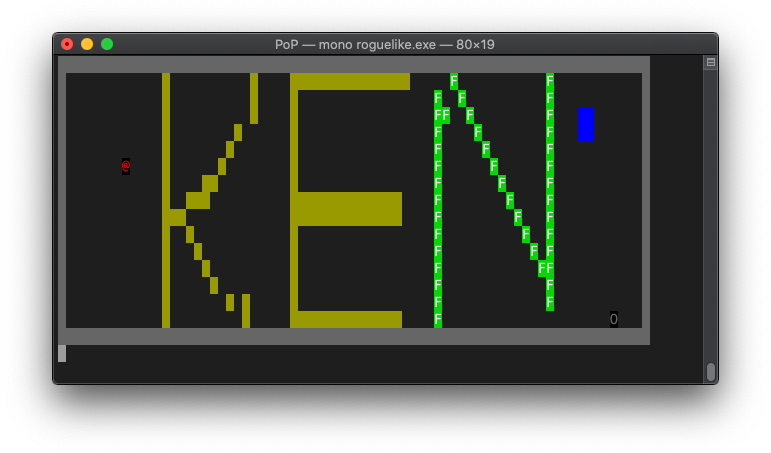
\includegraphics[width=.99\linewidth]{screenshot.png}

  \caption{Eksempel på hvordan spillet kunne se ud i terminalen. Den
    røde \texttt{@} er spilleren, resten er genstande og skabninger
    som spilleren kan interagere med (måske med fatale følger).}
  \label{fig:roguelike-screenshot}
\end{figure}

For at vise spillets verden implementerer vi en klasse
\lstinline{Canvas}, som er et gitter af felter. Hvor feltet
i øverste ventre hjørne har position $(0,0)$, og $x$-koordinatet
tælles op mod højre, og $y$-koordinatet tælles op når man bevæger sig
fra top mod bund.

Hvert felt har en \lstinline{char}, og så \emph{kan}
feltet have en forgrundsfarve, og det \emph{kan} have en baggrundsfarve.

Implementér klassen \lstinline{Canvas} som har følgende signatur:

\begin{lstlisting}
type Color = System.ConsoleColor
type Canvas =
  class
    new : rows:int * cols:int -> Canvas
    member Set: x:int * y:int * c:char * fg:Color * bg:Color -> unit
    member Show: unit -> unit
  end
\end{lstlisting}

Det vil sige:
\begin{itemize}
\item En konstruktør der tager antal rækker og koloner som argumenter.
%\item To properties der angiver det maksimale række-indeks, \lstinline{MaxX}, og
%  kolonne-indeks, \lstinline{MaxY}.
\item en metode \lstinline{Set} til at sætte indhold og farver på et
  felt.
\item en metode \lstinline{Show} til at vise en canvas i
  terminalen. Figur~\ref{fig:roguelike-screenshot} viser et eksempel
  på hvordan det kunne se ud.
\end{itemize}

I rapporten skal I beskrive jeres designovervejelser, samt redegøre
for hvilke data en canvas har.

\textbf{Hints}: Til \lstinline{Show} skal I bruge følgende
funktionalitet fra standard-biblioteket:

\begin{itemize}
\item \lstinline{System.Console.ForegroundColor <- System.ConsoleColor.White}
  til at sætte forgrundsfarven til hvid
  (kan også bruges til andre farver).
\item \lstinline{System.Console.BackgroundColor <- System.ConsoleColor.Blue}
  til at sætte baggrundsfarven til blå
  (kan også bruges til andre farver).
\item \lstinline{System.Console.ResetColor()} til at sætte farverne i
  terminalen tilbage til normal.
\end{itemize}


%%% Local Variables:
%%% mode: latex
%%% TeX-master: "main"
%%% End:
